% Options for packages loaded elsewhere
% Options for packages loaded elsewhere
\PassOptionsToPackage{unicode}{hyperref}
\PassOptionsToPackage{hyphens}{url}
\PassOptionsToPackage{dvipsnames,svgnames,x11names}{xcolor}
%
\documentclass[
  letterpaper,
  DIV=11,
  numbers=noendperiod]{scrartcl}
\usepackage{xcolor}
\usepackage{amsmath,amssymb}
\setcounter{secnumdepth}{-\maxdimen} % remove section numbering
\usepackage{iftex}
\ifPDFTeX
  \usepackage[T1]{fontenc}
  \usepackage[utf8]{inputenc}
  \usepackage{textcomp} % provide euro and other symbols
\else % if luatex or xetex
  \usepackage{unicode-math} % this also loads fontspec
  \defaultfontfeatures{Scale=MatchLowercase}
  \defaultfontfeatures[\rmfamily]{Ligatures=TeX,Scale=1}
\fi
\usepackage{lmodern}
\ifPDFTeX\else
  % xetex/luatex font selection
\fi
% Use upquote if available, for straight quotes in verbatim environments
\IfFileExists{upquote.sty}{\usepackage{upquote}}{}
\IfFileExists{microtype.sty}{% use microtype if available
  \usepackage[]{microtype}
  \UseMicrotypeSet[protrusion]{basicmath} % disable protrusion for tt fonts
}{}
\makeatletter
\@ifundefined{KOMAClassName}{% if non-KOMA class
  \IfFileExists{parskip.sty}{%
    \usepackage{parskip}
  }{% else
    \setlength{\parindent}{0pt}
    \setlength{\parskip}{6pt plus 2pt minus 1pt}}
}{% if KOMA class
  \KOMAoptions{parskip=half}}
\makeatother
% Make \paragraph and \subparagraph free-standing
\makeatletter
\ifx\paragraph\undefined\else
  \let\oldparagraph\paragraph
  \renewcommand{\paragraph}{
    \@ifstar
      \xxxParagraphStar
      \xxxParagraphNoStar
  }
  \newcommand{\xxxParagraphStar}[1]{\oldparagraph*{#1}\mbox{}}
  \newcommand{\xxxParagraphNoStar}[1]{\oldparagraph{#1}\mbox{}}
\fi
\ifx\subparagraph\undefined\else
  \let\oldsubparagraph\subparagraph
  \renewcommand{\subparagraph}{
    \@ifstar
      \xxxSubParagraphStar
      \xxxSubParagraphNoStar
  }
  \newcommand{\xxxSubParagraphStar}[1]{\oldsubparagraph*{#1}\mbox{}}
  \newcommand{\xxxSubParagraphNoStar}[1]{\oldsubparagraph{#1}\mbox{}}
\fi
\makeatother


\usepackage{longtable,booktabs,array}
\newcounter{none} % for unnumbered tables
\usepackage{calc} % for calculating minipage widths
% Correct order of tables after \paragraph or \subparagraph
\usepackage{etoolbox}
\makeatletter
\patchcmd\longtable{\par}{\if@noskipsec\mbox{}\fi\par}{}{}
\makeatother
% Allow footnotes in longtable head/foot
\IfFileExists{footnotehyper.sty}{\usepackage{footnotehyper}}{\usepackage{footnote}}
\makesavenoteenv{longtable}
\usepackage{graphicx}
\makeatletter
\newsavebox\pandoc@box
\newcommand*\pandocbounded[1]{% scales image to fit in text height/width
  \sbox\pandoc@box{#1}%
  \Gscale@div\@tempa{\textheight}{\dimexpr\ht\pandoc@box+\dp\pandoc@box\relax}%
  \Gscale@div\@tempb{\linewidth}{\wd\pandoc@box}%
  \ifdim\@tempb\p@<\@tempa\p@\let\@tempa\@tempb\fi% select the smaller of both
  \ifdim\@tempa\p@<\p@\scalebox{\@tempa}{\usebox\pandoc@box}%
  \else\usebox{\pandoc@box}%
  \fi%
}
% Set default figure placement to htbp
\def\fps@figure{htbp}
\makeatother


% definitions for citeproc citations
\NewDocumentCommand\citeproctext{}{}
\NewDocumentCommand\citeproc{mm}{%
  \begingroup\def\citeproctext{#2}\cite{#1}\endgroup}
\makeatletter
 % allow citations to break across lines
 \let\@cite@ofmt\@firstofone
 % avoid brackets around text for \cite:
 \def\@biblabel#1{}
 \def\@cite#1#2{{#1\if@tempswa , #2\fi}}
\makeatother
\newlength{\cslhangindent}
\setlength{\cslhangindent}{1.5em}
\newlength{\csllabelwidth}
\setlength{\csllabelwidth}{3em}
\newenvironment{CSLReferences}[2] % #1 hanging-indent, #2 entry-spacing
 {\begin{list}{}{%
  \setlength{\itemindent}{0pt}
  \setlength{\leftmargin}{0pt}
  \setlength{\parsep}{0pt}
  % turn on hanging indent if param 1 is 1
  \ifodd #1
   \setlength{\leftmargin}{\cslhangindent}
   \setlength{\itemindent}{-1\cslhangindent}
  \fi
  % set entry spacing
  \setlength{\itemsep}{#2\baselineskip}}}
 {\end{list}}
\usepackage{calc}
\newcommand{\CSLBlock}[1]{\hfill\break\parbox[t]{\linewidth}{\strut\ignorespaces#1\strut}}
\newcommand{\CSLLeftMargin}[1]{\parbox[t]{\csllabelwidth}{\strut#1\strut}}
\newcommand{\CSLRightInline}[1]{\parbox[t]{\linewidth - \csllabelwidth}{\strut#1\strut}}
\newcommand{\CSLIndent}[1]{\hspace{\cslhangindent}#1}



\setlength{\emergencystretch}{3em} % prevent overfull lines

\providecommand{\tightlist}{%
  \setlength{\itemsep}{0pt}\setlength{\parskip}{0pt}}



 


\KOMAoption{captions}{tableheading}
\setlength{\parindent}{15pt}
\setlength{\parskip}{0pt}
\makeatletter
\@ifpackageloaded{caption}{}{\usepackage{caption}}
\AtBeginDocument{%
\ifdefined\contentsname
  \renewcommand*\contentsname{Table of contents}
\else
  \newcommand\contentsname{Table of contents}
\fi
\ifdefined\listfigurename
  \renewcommand*\listfigurename{List of Figures}
\else
  \newcommand\listfigurename{List of Figures}
\fi
\ifdefined\listtablename
  \renewcommand*\listtablename{List of Tables}
\else
  \newcommand\listtablename{List of Tables}
\fi
\ifdefined\figurename
  \renewcommand*\figurename{Figure}
\else
  \newcommand\figurename{Figure}
\fi
\ifdefined\tablename
  \renewcommand*\tablename{Table}
\else
  \newcommand\tablename{Table}
\fi
}
\@ifpackageloaded{float}{}{\usepackage{float}}
\floatstyle{ruled}
\@ifundefined{c@chapter}{\newfloat{codelisting}{h}{lop}}{\newfloat{codelisting}{h}{lop}[chapter]}
\floatname{codelisting}{Listing}
\newcommand*\listoflistings{\listof{codelisting}{List of Listings}}
\makeatother
\makeatletter
\makeatother
\makeatletter
\@ifpackageloaded{caption}{}{\usepackage{caption}}
\@ifpackageloaded{subcaption}{}{\usepackage{subcaption}}
\makeatother
\usepackage{bookmark}
\IfFileExists{xurl.sty}{\usepackage{xurl}}{} % add URL line breaks if available
\urlstyle{same}
\hypersetup{
  pdftitle={Tutorial: Marginal Structural Models for Panel Conditioning Research},
  pdfauthor={Luca Y. Kogelheide},
  colorlinks=true,
  linkcolor={blue},
  filecolor={Maroon},
  citecolor={Blue},
  urlcolor={Blue},
  pdfcreator={LaTeX via pandoc}}


\title{Tutorial: Marginal Structural Models for Panel Conditioning
Research}
\author{Luca Y. Kogelheide}
\date{15.06.2026}
\begin{document}
\maketitle


This simulation is based on a paper by Blackwell \& Glynn (2018). You
can find the Dataverse and replication files
\href{https://dataverse.harvard.edu/dataset.xhtml?persistentId=doi:10.7910/DVN/SFBX6Z}{here}.

\section{Why Marginal Structural
Models?}\label{why-marginal-structural-models}

Let's assume we are interested in the longitudinal effect of a
particular treatment \(A(t)\). This treatment could be the intake of a
specific medicine, taking part in a training programme, or participating
in some sort of event -- like participating in a survey. In addition to
treatment \(t\), we also measure other predictors stored in the vector
\(L(z)\). Let \(\bar A(t)\) be the treatment history and \(\bar L(z)\)
the history of predictors.

According, to Robins (1999), say that a treatment process is
\emph{causally exogenous} when the conditional probability of receiving
treatment at time-point \(k\) given past treatment and prognostic
factors (predictors) only depends on past treatment history,
i.e.~\(\Pr(A(t_k) \mid \bar A(t); \bar L(z)) = \Pr(A(t_k) \mid \bar A(t))\).
Translating this to \emph{statistical exogeneity} means that the
probability of receiving treatment at time-point \(k\) does not depend
on the history of measured time-dependent predictors \(\bar L(z)\) up to
\(k\), conditional on treatment history prior to \(k\):

\[
A(t_k) \perp \!\!\! \perp \bar L(t_k) \mid \bar A(t_{k-1}).
\] In this case we can run a simple regression to identify the causal
effect of treatment on the outcome:
\(\mathbb{E}[Y \mid \bar A] = \beta_0 + \beta_1 \text{cum}(A)\), where
\(\text{cum}(A)\) is the individual cumulative treatment.

However, this is quite a strong assumption, and often times the
treatment does depend on (measured) covariates that also predict the
outcome, a process known as time-varying confounding. We talk about
\emph{time-varying confounding} if a time-varying predictor \(z_k\) is a
predictor of the outcome of interest \(Y_k\) and also predicts
subsequent treatment exposure \(A(t_{k+1})\). Furthermore, when
treatment is not only influenced by previous levels of the covariates,
but also causally affects future levels of the covariates, \(L(z)\) is a
time-varying confounder affected by prior treatment. We call this
\emph{treatment-induced time-varying confounding}, or
treatment-confounder feedback (Robins et al., 2000). Including
covariates which are influenced by prior treatment into the model blocks
part of the causal effect of \(A(t)\) on \(Y\), introducing
post-treatment bias into the regression estimates. Now, the relevant
predictors are not only confounders, which we usually want to control
for in our model, but also affected by prior treatment, which introduces
post treatment bias if included in the model. Marginal Structural Models
(MSMs) solve this by using inverse-probability-of-treatment weighting to
create a pseudo-population where treatment is no longer associated with
those confounders.

\subsection{Treatment-Induced Time-Varying Confounding in Panel
Conditioning
Research}\label{treatment-induced-time-varying-confounding-in-panel-conditioning-research}

Relating this to the study of panel conditioning, we have survey
participation as treatment, and misreporting behaviour in future survey
waves as the outcome of interest. The causal exogeneity condition would
be: The probability of participating in the survey at wave \(k\), given
past participation and respondent characteristics, depends only on past
participation history, not on respondent's characteristics. This is
obviously unrealistic, as we would assume that some respondent's
characteristics are related to both misreporting and survey
participation: subjective response burden, susceptibility to social
desirability, survey experience, or trust in the survey/institution.
Similarly, it is reasonable to assume that at least some of these
characteristics are also influenced by survey participation, making them
treatment-induced time-varying confounders.

\section{Introducing Marginal Structural
Models}\label{introducing-marginal-structural-models}

Building on the \emph{Potential Outcomes Framework}, we define
\(Y_{\bar a}\) to be the (possibly counterfactual) random variable
representing a subject's outcome had the subject been treated with
treatment history \(\bar a = \{a(t); 0 \leq t \leq K+1 \}\), instead of
his/her observed history \(\bar A\). We define
\(\mathbb{E}[Y_{\bar a}] = \beta_0 + \beta_1 \text{cum}(\bar a)\) as our
marginal structural model --- a model for the marginal distribution of
each counterfactual outcome (Robins, 1999). Let's say our outcome
variable is binary. We want to model the marginal outcome probability as

\[\Pr(Y_{\bar a} = 1) = \beta_0 + \beta_1 \text{cum}(\bar a).\]

However, using observed data we can only model

\[\Pr(Y = 1 \mid \bar A = \bar a) = \gamma_0 + \gamma_1 \text{cum}(\bar a),\]

as we only observe treatment history \(\bar A\). \(\beta_1 = \gamma_1\)
is only true when complete causal exogeneity holds. Otherwise, we can
use a weighted regression approach to obtain an unbiased estimate of
\(\beta_1\). Assuming we have measured all relevant predictors \(L(z)\),
we can create a pseudo-population in which, after weighting, the
confounders are equally distributed across the treated and the untreated
groups (Chesnaye et al., 2022) and thus can be interpreted as if it
arose from a sequentially randomized trial. The
inverse-probability-of-treatment weight (IPTW) models each subjects'
probability of having his/her own observed treatment history (propensity
score) and taking the inverse of this probability:

\[w_i = \left[\prod_{k=0}^K \Pr(A_k = a_{ki} \mid \bar A_{k-1} = \bar a_{k-1, i}, \bar L_k)\right]^{-1}.\]
To reduce its variance, we can further stabilize these IPTWs by
including their baseline probability in the numerator of the weighting
model:

\[sw_i = \prod_{k=0}^K\frac{\Pr(A_k = a_{ki} \mid \bar A_{k-1} = \bar a_{k-1, i}} {\Pr(A_k = a_{ki} \mid \bar A_{k-1} = \bar a_{k-1, i}, \bar L_k)}.\]
The numerator conditions only on past treatment, producing a
pseudo-population in which participation at wave \(k\) is independent of
the time-varying confounders given past participation history (Robins,
1999). The denominator model additionally conditions on the confounders,
removing the dependence from the observed data.\\
Furthermore, it is good practice to truncate the weights (usually at the
1st and 99th percentile or at the 5th and 95th percentile) to remove
larger outliers and thus reduce the weights variance (Cole \& Hernán,
2008).

\subsection{Representing Treatment-Induced Time-Varying Confounding
Using Directed Acyclic
Graphs}\label{representing-treatment-induced-time-varying-confounding-using-directed-acyclic-graphs}

We can represent such a data-generating process (DGP) in which we have
treatment-induced time-varying confounding as follows. To repeat: We
talk about time-varying confounding, if

\begin{itemize}
\tightlist
\item
  a time-varying predictor \(z_k\) is a predictor of the outcome of
  interest \(Y_k\), and\\
\item
  a time-varying predictor \(z_k\) is a predictor of subsequent
  treatment exposure \(A(t_{k+1}).\)
\end{itemize}

We can visualize this using directed acyclic graphs (DAGs). To make it
easier to interpret, we restrict the DAG to two time-points: \(k-1\) and
\(k\). This can easily be extended to any number of time-points.

\pandocbounded{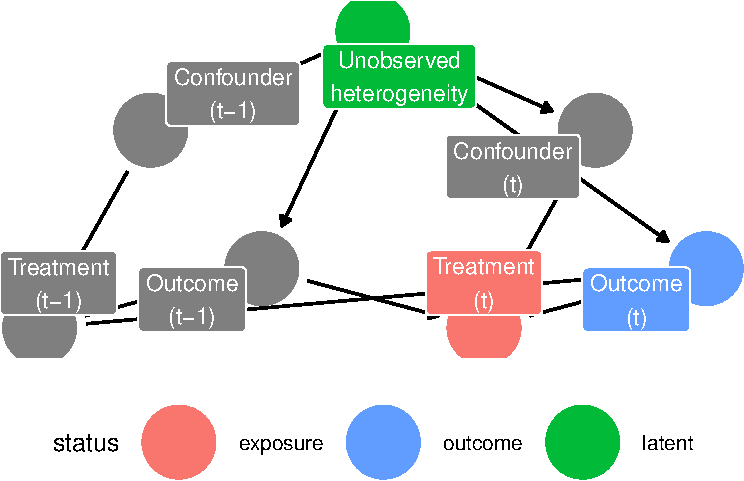
\includegraphics[keepaspectratio]{MSMPanelCond_files/figure-pdf/unnamed-chunk-2-1.pdf}}

In this DAG, we see that the confounders are a causal predictor of
treatment, and treatment is a causal predictor of the outcome variable
of interest. Furthermore, the outcome variable at the previous
time-point is a direct cause of the treatment variable at the next
time-point. Note that the confounder variable does not have a direct
causal relationship with our outcome variable. However, because both
have a common cause, namely unobserved heterogeneity, they are
correlated due to an indirect relationship and the confounder is a
meaningful predictor of the outcome variable. In the simulation, I will
also include a scenario in which there is such a direct causal
relationship.

Additionally, we talk about treatment-induced time-varying confounding,
if

\begin{itemize}
\tightlist
\item
  we have time-varying confounding, and\\
\item
  treatment \(A(t_k)\) causally affects subsequent levels of the
  covariates \(z_{k+1}\) (see the arrow from ``Treatment (t-1)'' to
  ``Confounder (t)'').
\end{itemize}

\pandocbounded{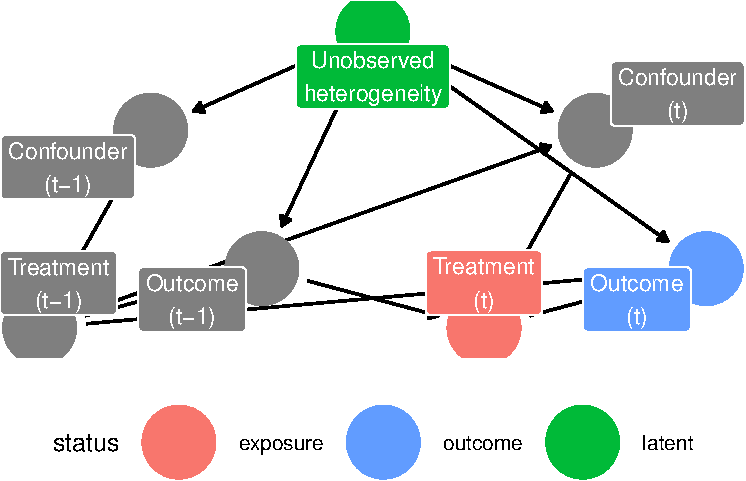
\includegraphics[keepaspectratio]{MSMPanelCond_files/figure-pdf/unnamed-chunk-3-1.pdf}}

Lastly, we can also include a direct causal effect from the confounder
(in our case respondents characteristics) to our outcome variable of
interest.

\pandocbounded{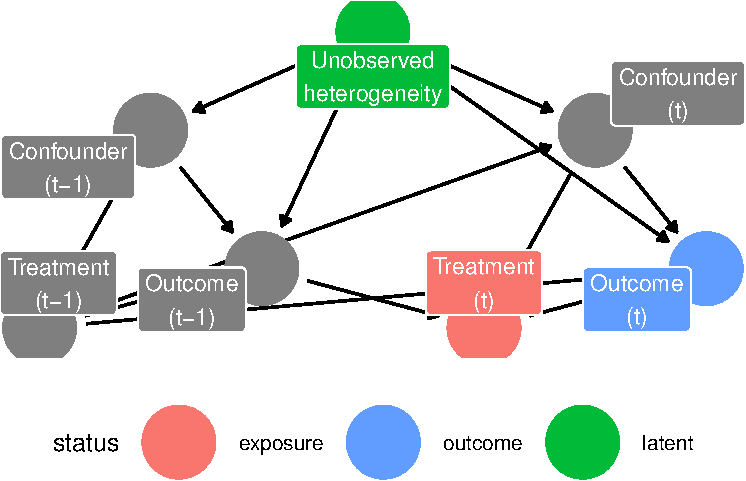
\includegraphics[keepaspectratio]{MSMPanelCond_files/figure-pdf/unnamed-chunk-4-1.pdf}}

\section{Simulation:}\label{simulation}

\subsection{The Data-Generating
Process}\label{the-data-generating-process}

To build intuition for what MSMs do and when they are needed, we build
upon and extend the simulated panel dataset of
\href{https://www.cambridge.org/core/journals/american-political-science-review/article/abs/how-to-make-causal-inferences-with-timeseries-crosssectional-data-under-selection-on-observables/498BE04E5AF9802EC4D33DD7A4016584}{Blackwell
\& Glynn (2018)} in which we know the true causal structure by
construction. We generate data for \(100\) and \(1500\) respondents
observed over \(5\) time periods (survey waves). At each wave, three
variables are recorded, a time-varying confounder \(z_{ik}\), a binary
treatment indicator \(x_{ik}\), and a continuous outcome \(y_{ik}\)
serving as a latent measure of misreporting propensity. The simulation
also tracks four potential outcomes:
\(y_{ik}^{11}, y_{ik}^{10}, y_{ik}^{01}, y_{ik}^{00}\), where the
superscripts denote whether the respondents participated in the previous
wave and the current wave, respectively.

\subsubsection{Unobserved Heterogeneity}\label{unobserved-heterogeneity}

To capture stable between-person differences, each respondent is
assigned a time-stable unobserved characteristic
\(u_i \sim \mathcal{N}(0, \sigma),\) with \(\sigma\) = 0.1. Unobserved
heterogeneity influences both participation decisions and reporting
behaviour throughout the panel. Because \(u_i\) is never observed, it
acts as a latent common cause of treatment and outcome at every wave,
opening backdoor paths that cannot be closed by conditioning on measured
covariates alone. Thus, it is to be expected that we find some bias in
our models later on.

\subsubsection{Time-Varying Confounder}\label{time-varying-confounder}

We initialize the confounder as
\[ z_{i1} = 1.7u_i + \varepsilon_{i1}^z, \quad \varepsilon_{i1}^z \sim \mathcal{N}(-0.4, \sigma). \]
At all subsequent waves, the confounder evolves according to treatment
status at the previous wave:
\[ z_{ik} = \gamma_1 + \gamma_2x_{i, k-1} + 1.7u_i + \varepsilon_{i1}^z, \quad \varepsilon_{i1}^z \sim \mathcal{N}(0, \sigma), \]
with \(\gamma_1\) = 0.5 and \(\gamma_2\) = 0 in the scenario
\emph{without} treatment-induced confounding and \(\gamma_2\) = -0.5 in
the scenario \emph{with} treatment-induced confounding. Standard
covariate adjustment breaks down here, because conditioning on
\(z_{ik}\) to remove confounding simultaneously blocks part of the
causal effect that runs through the treatment-confounder-outcome chain,
making MSMs necessary. In our case, participating at wave \(k-1\)
changes the respondents state which then predicts both their probability
of participating again and how they report in the future.

\subsubsection{Treatment Assignment}\label{treatment-assignment}

At the first wave, treatment is binary and follows a logistic model:
\[\Pr(x_{i1} = 1) = \text{logit}^{-1}(\alpha_0 + \alpha_1z_{i1}),\] with
intercept \(\alpha_0\) = -2.5 and coefficient \(\alpha_1\) = 1.5. From
wave 2 onward, participation is modelled as a latent-variable probit:
\[ x_{ik} = 1[\alpha_0 + \alpha_1z_{ik} + \alpha_2y_{i, k-1} + \nu_{ik} > 0] \quad \nu_{ik} \sim \mathcal{N}(0,1), \]
with \(\alpha_0\) = -2.5, \(\alpha_1\) = 1.5, and \(\alpha_2\) = -1.
Next to the current confounder \(z_{ik}\), we see that \emph{lagged
outcome} \(y_{i, k-1}\) predicts the participation propensity. This
creates a causal relationship from past outcome to future treatment in
the DAG and is the pathway through which non-ignorable attrition
operates in this simulation.

\subsubsection{Outcome Variable}\label{outcome-variable}

The outcome at wave 1 is drawn from a baseline level that depends on
unobserved heterogeneity, the confounder, and whether the respondent was
treated:
\[ y_{i1} = 0.8 + 0.9u_i + \eta z_{i1} + \mu x_{i1} + \varepsilon_{i1}^y, \]
where \(\eta\) = 0 in the scenario where the confounder has no direct
effect on the outcome, \(\eta\) = 0.3 when the confounder has a direct
effect, and \(\mu\) = -0.15 is the contemporaneous effect of being
treated for the first time. From wave 2 onward, the outcome is defined
through a potential-outcomes decomposition: \[ 
y_{ik} = y_{ik}^{00} + x_{i,k-1}\underbrace{(y_{ik}^{10}-y_{ik}^{00})}_{\text{lagged effect}} + 
x_{ik}\underbrace{(y_{ik}^{01}-y_{ik}^{00})}_{\text{contemp. effect}} +
x_{i,k-1}x_{ik}\underbrace{[(y_{ik}^{11}-y_{ik}^{01})-(y_{ik}^{10}-y_{ik}^{00})]}_{\text{interaction}}.
\] The four potential outcomes are constructed additively from the
baseline, the lagged effect \(\mu_0\) = 0.1, the contemporaneous effect
\(\mu_1\) = -0.25 (participated in both current and previous wave) and
\(\mu_2\) = -0.15 (participated in current wave only), all relative to
the untreated baseline \(y_{ik}^{00}.\)

\subsection{Model and Identification
Strategies}\label{model-and-identification-strategies}

Using this DGP I want to compare how different models recover the true
causal effects. For each simulated dataset, we estimate 12 models,
ranging from naive regression to several variants of MSM estimators, and
evaluate each by its bias relative to the known true value and its RMSE
(root mean squared error).

\subsubsection{Estimands}\label{estimands}

We target two distinct causal quantities, both computed as average
treatment effects (ATEs) over waves \(k \geq 2\) to allow at least one
lag to be defined:
\begin{align*}
\tau_{\text{lagged}} = \mathbb{E}[y_{ik}^{10}-y_{ik}^{00}] \\
\tau_{\text{current}} = \mathbb{E}[y_{ik}^{11}-y_{ik}^{10}]
\end{align*}
The first, \(\tau_{\text{lagged}}\), is the effect of having been
treated at the \emph{previous} wave while untreated at the current wave,
relative to no treatment at either wave. The second,
\(\tau_{\text{current}}\), is the \emph{additional} effect of being
treated now, given that one was already treated at the previous wave.
While naive regression approaches are usually not able to separate these
two quantities, ADL (autoregressive distributed lag) models and MSMs
can. We thus compare different specifications of these three classes of
models.

\subsubsection{Benchmark Regressions}\label{benchmark-regressions}

We have a total of 6 regression approaches. We include one naive simple
regression which ignores all confounding as a benchmark, and one
regression which includes \(z_{ik}\) as a confounder.\\
Additionally, we include 4 ADL models, which can additionally include
lags of the outcome, the treatment, and/or the confounder. The idea of
autoregressive distributed lag models is to include \(y_{i, k-1}\) as a
regressor to account for stable unobserved heterogeneity, and by
including \(x_{i, k-1}\) as a regressor to get an estimate of a lagged
treatment/participation effect. However, as we discussed above, this
usually introduces post treatment bias into the estimate.\\
Note that, for the ADL models, the lagged treatment effect is not simply
the coefficient on \(x_{i,k-1}\), because \(y_{i,k-1}\) is also in the
model and also depends on \(x_{i,k-1}\). To recover the total lagged
effect, our ADL estimate is
\[ \tau_{\text{lagged}}^{\text{ADL}} = \hat\beta_{x_{k-1}} +\hat\beta_{y_{k-1}}\cdot \hat\beta_{x_k}. \]

\begin{longtable}[]{@{}
  >{\raggedright\arraybackslash}p{(\linewidth - 2\tabcolsep) * \real{0.3118}}
  >{\raggedright\arraybackslash}p{(\linewidth - 2\tabcolsep) * \real{0.6882}}@{}}
\caption{Included Autoregressive Distributed Lag Models}\tabularnewline
\toprule\noalign{}
\begin{minipage}[b]{\linewidth}\raggedright
Model
\end{minipage} & \begin{minipage}[b]{\linewidth}\raggedright
Regressors
\end{minipage} \\
\midrule\noalign{}
\endfirsthead
\toprule\noalign{}
\begin{minipage}[b]{\linewidth}\raggedright
Model
\end{minipage} & \begin{minipage}[b]{\linewidth}\raggedright
Regressors
\end{minipage} \\
\midrule\noalign{}
\endhead
\bottomrule\noalign{}
\endlastfoot
ADL (1) & \(x_{ik}, x_{i,k-1}, y_{i,k-1}\) \\
ADL (1) + cont. confounder & \(x_{ik}, x_{i,k-1}, y_{i,k-1}, z_{ik}\) \\
ADL (1) + lagged confounder &
\(x_{ik}, x_{i,k-1}, y_{i,k-1}, z_{ik}, z_{i,k-1}\) \\
ADL (2) &
\(x_{ik}, x_{i,k-1}, y_{i,k-1}, y_{i,k-2}, z_{ik}, z_{i,k-1}\) \\
\end{longtable}

\subsubsection{Inverser-Probability-of-Treamtent
Weights}\label{inverser-probability-of-treamtent-weights}

The MSMs all share a GEE (generalized estimating equations) regression
of \(y_{ik}\) on current treatment \(x_{ik}\) and lagged treatment
\(x_{i,k-1}\), estimated under working independence, as the outcome
model to account for autocorrelation of the panel data. They only differ
in how the stabilized weights are constructed. We estimate three
stabilized weight specifications, each with both raw and truncated
variants (truncation at the 5th and 95th percentile). Cumulative
stabilized weights are of the general form:
\[ \tilde w_{ik} = \prod_{s=1}^K \frac{\Pr(x_{is} \mid \bar x_{i, s-1})}{\Pr(x_{is} \mid \bar x_{i, s-1}, \bar z_{is}, y_{i, s-1})}, \]
where \(\bar x_{i, s-1}\) and \(\bar z_{is}\) denote the history of
treatment and confounder up to the relevant wave. They only differ in
how many lags are included into the model. Both numerator and
denominator are estimated via logistic regression and the resulting
probability scores are converted to observation-level weights by taking
their fitted probabilities.

{\def\LTcaptype{none} % do not increment counter
\begin{longtable}[]{@{}
  >{\raggedright\arraybackslash}p{(\linewidth - 4\tabcolsep) * \real{0.3793}}
  >{\raggedright\arraybackslash}p{(\linewidth - 4\tabcolsep) * \real{0.3276}}
  >{\raggedright\arraybackslash}p{(\linewidth - 4\tabcolsep) * \real{0.2931}}@{}}
\toprule\noalign{}
\begin{minipage}[b]{\linewidth}\raggedright
Weight specification
\end{minipage} & \begin{minipage}[b]{\linewidth}\raggedright
Denominator model
\end{minipage} & \begin{minipage}[b]{\linewidth}\raggedright
Numerator model
\end{minipage} \\
\midrule\noalign{}
\endhead
\bottomrule\noalign{}
\endlastfoot
\textbf{1-lag} & \(x_{it} \sim y_{i,t-1} + z_{it} + x_{i,t-1}\) &
\(x_{it} \sim x_{i,t-1}\) \\
\textbf{2-lag} &
\(x_{it} \sim y_{i,t-1} + z_{it} + x_{i,t-1} + y_{i,t-2} + z_{i,t-1} + x_{i,t-2}\)
& \(x_{it} \sim x_{i,t-1} + x_{i,t-2}\) \\
\textbf{Cumulative} &
\(x_{it} \sim y_{i,t-1} + z_{it} + x_{i,t-1} + \widetilde{X}_{i,t-2}\) &
\(x_{it} \sim x_{i,t-1} + \widetilde{X}_{i,t-2}\) \\
\end{longtable}
}

where \(\bar X_{i, t-2}\) denotes cumulative prior treatment exposure up
to two waves before the current one.

\subsection{Results}\label{results}

We run this simulation as a Monte-Carlo simulation with 1000 iterations
for each of the four DGP scenarios

\subsubsection{Absolute Bias}\label{absolute-bias}

For each of the twelve models, performance is summarized by the bias
relative to the true ATE:
\begin{align*}
\text{Bias}_{\text{current}} = \tau_{\text{current}} - \hat \tau_{\text{current}} \\
\text{Bias}_{\text{lagged}} = \tau_{\text{lagged}} - \hat \tau_{\text{lagged}}.
\end{align*}
Note that the two naive regression models do not yield a lagged effect
estimate.

\pandocbounded{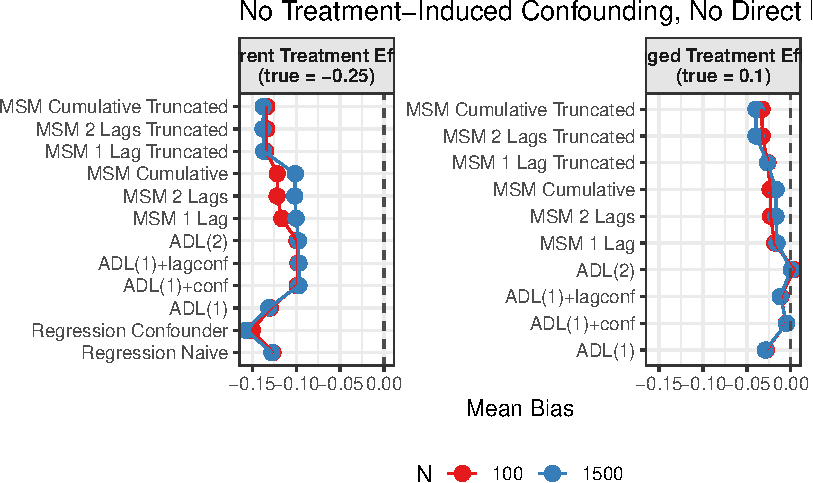
\includegraphics[keepaspectratio]{MSMPanelCond_files/figure-pdf/unnamed-chunk-5-1.pdf}}

\pandocbounded{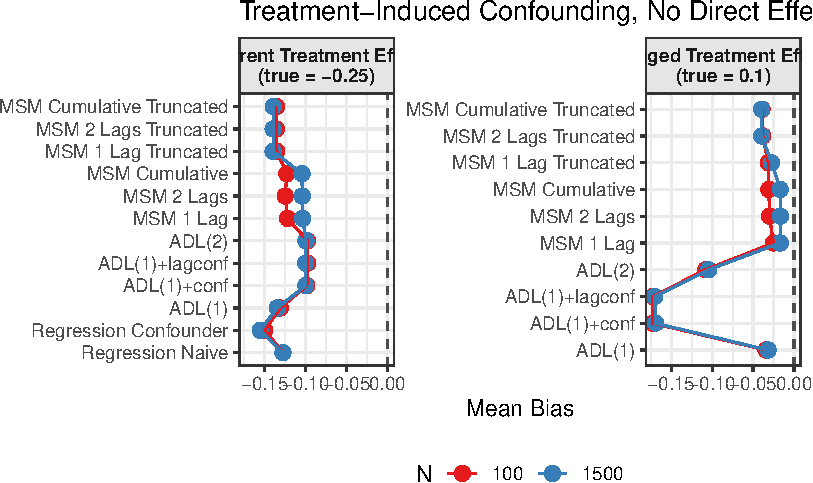
\includegraphics[keepaspectratio]{MSMPanelCond_files/figure-pdf/unnamed-chunk-6-1.pdf}}

\pandocbounded{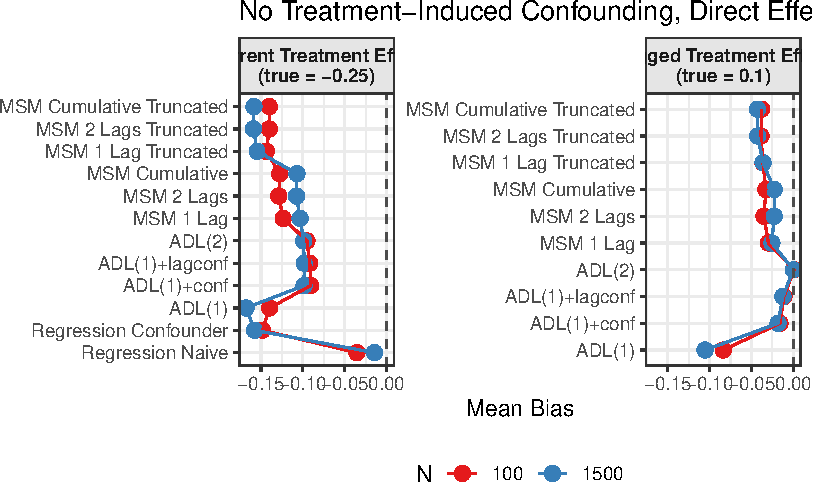
\includegraphics[keepaspectratio]{MSMPanelCond_files/figure-pdf/unnamed-chunk-7-1.pdf}}

\pandocbounded{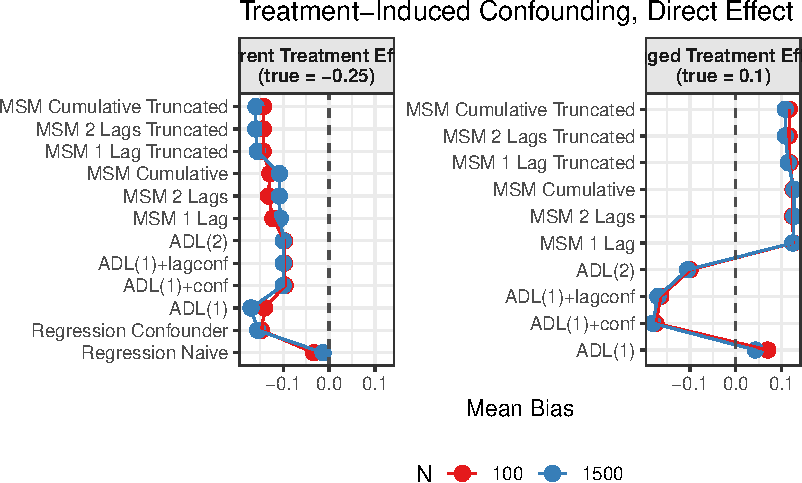
\includegraphics[keepaspectratio]{MSMPanelCond_files/figure-pdf/unnamed-chunk-8-1.pdf}}

\subsubsection{Root Mean Squared Error}\label{root-mean-squared-error}

In additional to absolute mean bias, we also want to measure how far
estimates scatter around the true value on average, regardless of
direction. We therefore also calculate the RMSE (root mean squared
error):

\[
\begin{split}
\mathrm{RMSE} &= \sqrt{\mathrm{Bias}^2+\mathrm{Variance}} \\
              &= \sqrt{\frac{1}{B} \sum_{b=1}^B (\hat\tau_b - \tau)^2}, 
\end{split}
\] where \(B\) = 1000 is the number of Monte-Carlo iterations,
\(\hat\tau_b\) is the estimate from replication \(b\), and \(\tau\) is
the true effect.

\pandocbounded{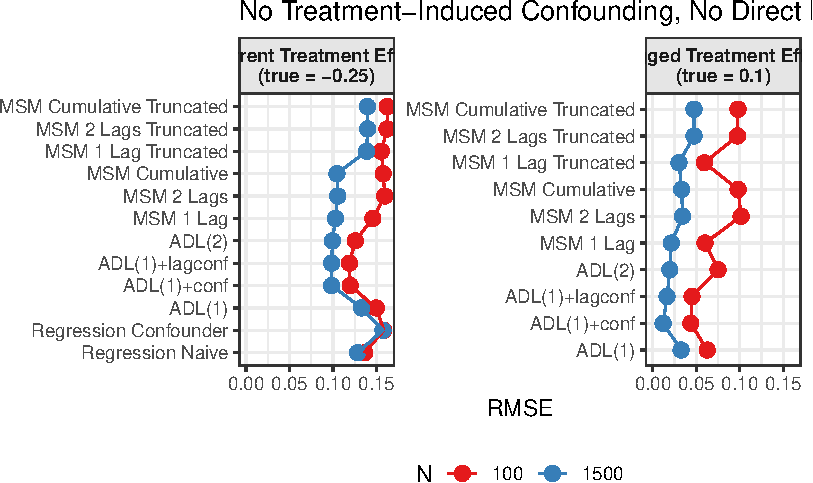
\includegraphics[keepaspectratio]{MSMPanelCond_files/figure-pdf/unnamed-chunk-9-1.pdf}}

\pandocbounded{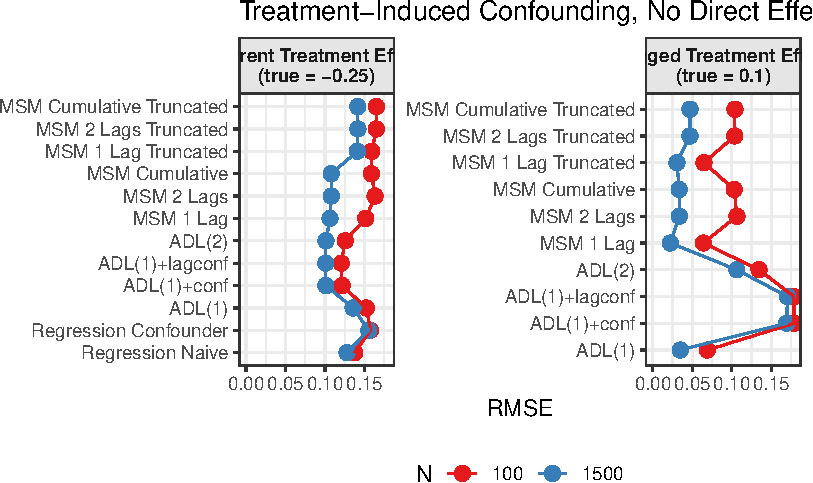
\includegraphics[keepaspectratio]{MSMPanelCond_files/figure-pdf/unnamed-chunk-10-1.pdf}}

\pandocbounded{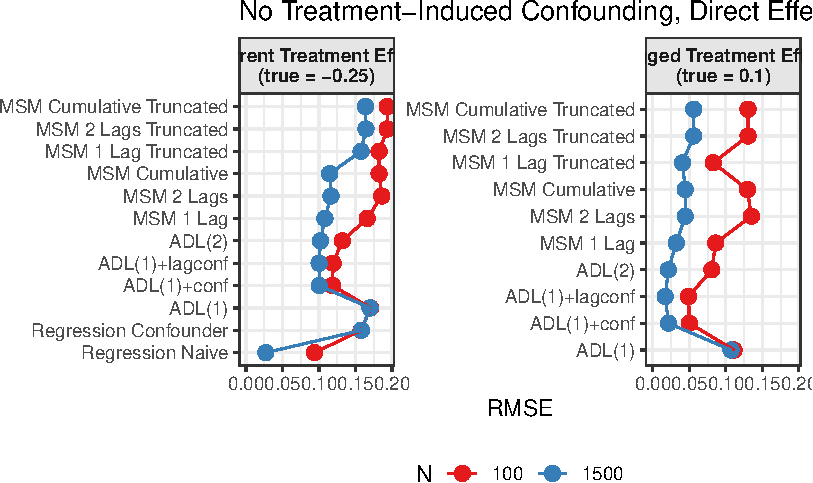
\includegraphics[keepaspectratio]{MSMPanelCond_files/figure-pdf/unnamed-chunk-11-1.pdf}}

\pandocbounded{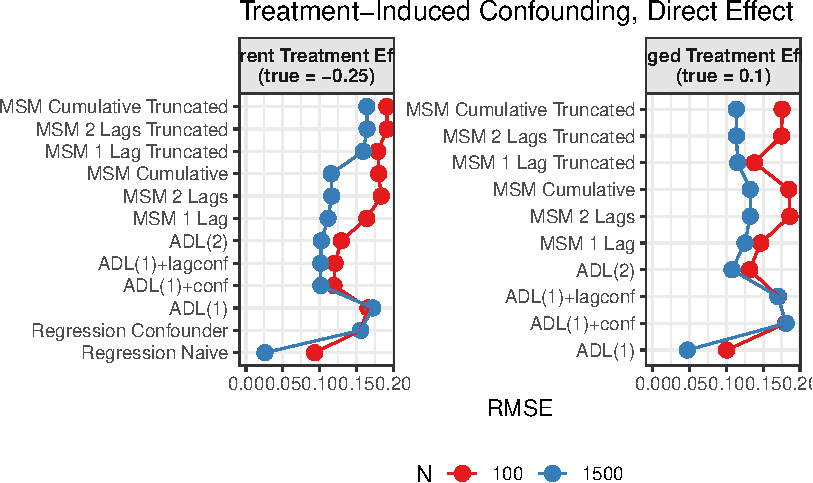
\includegraphics[keepaspectratio]{MSMPanelCond_files/figure-pdf/unnamed-chunk-12-1.pdf}}

\subsubsection{Discussion}\label{discussion}

Since we are specifically interested in the effect of participation in
previous survey waves on current misreporting propensity, we mostly care
about performance of the lagged effect estimates when there is
treatment-induced time-varying confounding (figures 2 and 4).

In general, we see that in terms of bias, we get less biased results for
the lagged effect compared to the current treatment effects. We also see
that MSMs generally outperform ADLs in scenarios with treatment-induced
time-varying confounding.

We see similar results in terms of RMSE. Lagged treatment effects are
more accurate than current treatment effects and MSMs generally perform
better in cases of treatment-induced time-varying confounders compared
to ADLs. While sometimes ADL models perform quite well (e.g.~ADL (1)),
MSMs seem to be less prone to model misspecification.

All in all, based on these results, I would prefer MSMs to ADL models,
since model specification seems to be influencing ADL models more
strongly and misspecification might become an issue. MSMs all perform
reasonably well, even though they seem to struggle somewhat in cases
with strong treatment-induced confounding and direct causal effects of
time-varying confounders on the outcome variable.

\section*{References}\label{references}
\addcontentsline{toc}{section}{References}

\protect\phantomsection\label{refs}
\begin{CSLReferences}{1}{0}
\bibitem[\citeproctext]{ref-blackwell2018make}
Blackwell, M., \& Glynn, A. N. (2018). How to make causal inferences
with time-series cross-sectional data under selection on observables.
\emph{American Political Science Review}, \emph{112}(4), 1067--1082.
\href{https://doi.org/10.1017/S0003055418000357\%20}{https://doi.org/10.1017/S0003055418000357
}

\bibitem[\citeproctext]{ref-chesnaye2022introduction}
Chesnaye, N. C., Stel, V. S., Tripepi, G., Dekker, F. W., Fu, E. L.,
Zoccali, C., \& Jager, K. J. (2022). An introduction to inverse
probability of treatment weighting in observational research.
\emph{Clinical Kidney Journal}, \emph{15}(1), 14--20.
\url{https://doi.org/10.1093/ckj/sfab158}

\bibitem[\citeproctext]{ref-cole2008constructing}
Cole, S. R., \& Hernán, M. A. (2008). Constructing inverse probability
weights for marginal structural models. \emph{American Journal of
Epidemiology}, \emph{168}(6), 656--664.
\url{https://doi.org/10.1093/aje/kwn164}

\bibitem[\citeproctext]{ref-robins1999association}
Robins, J. M. (1999). Association, causation, and marginal structural
models. \emph{Synthese}, \emph{121}(1/2), 151--179.

\bibitem[\citeproctext]{ref-robins2000marginal}
Robins, J. M., Hernan, M. A., \& Brumback, B. (2000). Marginal
structural models and causal inference in epidemiology. In
\emph{Epidemiology} (No. 5; Vol. 11, pp. 550--560). Lww.

\end{CSLReferences}




\end{document}
